\section{Proposed implementation}
Following the proposed architecture, presented in the previous chapter, we will now explain the actual implementation we performed to achieve our goals.
This section briefly presents the overall idea and proposed system architecture without going into details about specific choices.
Those explanations will be presented in later sections, as we will delve deeper into the implementation details, including product and technology choices, both in terms of hardware and software.

\subsection{Master node}
The master node of our system will be implemented in a generic desktop PC through the usage of an industrial programming platform.
This will enable us to program the behaviour of the master node as well as provide the necessary communication libraries to implement a master node for different RTE networks.
We will take advantage of the fact that most industrial programming platforms allow us to determine the RTE network's update period.
This will enable us to perform tests using different network cycle times.

Two programs will be developed for the master node:
\begin{enumerate}
	\item one to act as a simple set-point generator, sending the velocity or position set-points to the slave device through the RTE network;
	\item a second one to act as the motion controller, where the same set-points are used internally in a control algorithm that receives the plant feedback value and sends the plant output value through the RTE network.
\end{enumerate}

This implementation will allow us to perform the two practical experiments described in \autoref{sec:experiments}, enabling us to compare performance values acquired in both cases.

\subsection{Slave node}
The proposed slave implementation will be based on an embedded computing platform.
The embedded platform will be extended using some specialised boards that will broaden the functionality of the slave device as a whole.
These extension will provide easier access to the GPIO pins, direct interface with a motor through a specialised DC motor control board and Real-Time Ethernet connection using a dedicated board capable of off-loading the real-time processing of network packets from the embedded computing platform.

Additionally, in order to create a connection with the real world, we'll be using a DC motor paired with an incremental encoder.
This will allow data to be collected from a real world source, giving a more organic feeling to the process of running experiments with this system.

In terms of software, a control application will be developed for the slave device computing platform in order to provide the following functionality on the slave device:
\begin{itemize}
	\item Handle the receiving and sending of cyclic data through the RTE network by interfacing with the driver of the dedicated RTE network connection board. Such data will include set-point and feedback values;
	\item Handle the plant feedback signals, converting them into internal variables.;
	\item Handle the motor output signal by interfacing with the dedicated DC motor control board;
	\item Acquire and export performance data relating to the control of the DC motor speed and/or position;
	\item Provide an internal control algorithm to locally control the motor's speed and/or position;
\end{itemize}

Such software will be implemented in modules, and a general overview of how they interconnect with each other can be seen in a block diagram format in \autoref{fig:sw-architecture}.
The block names represent the actual names used for the different modules that were implemented.

\begin{figure}[htp]
	\centering
	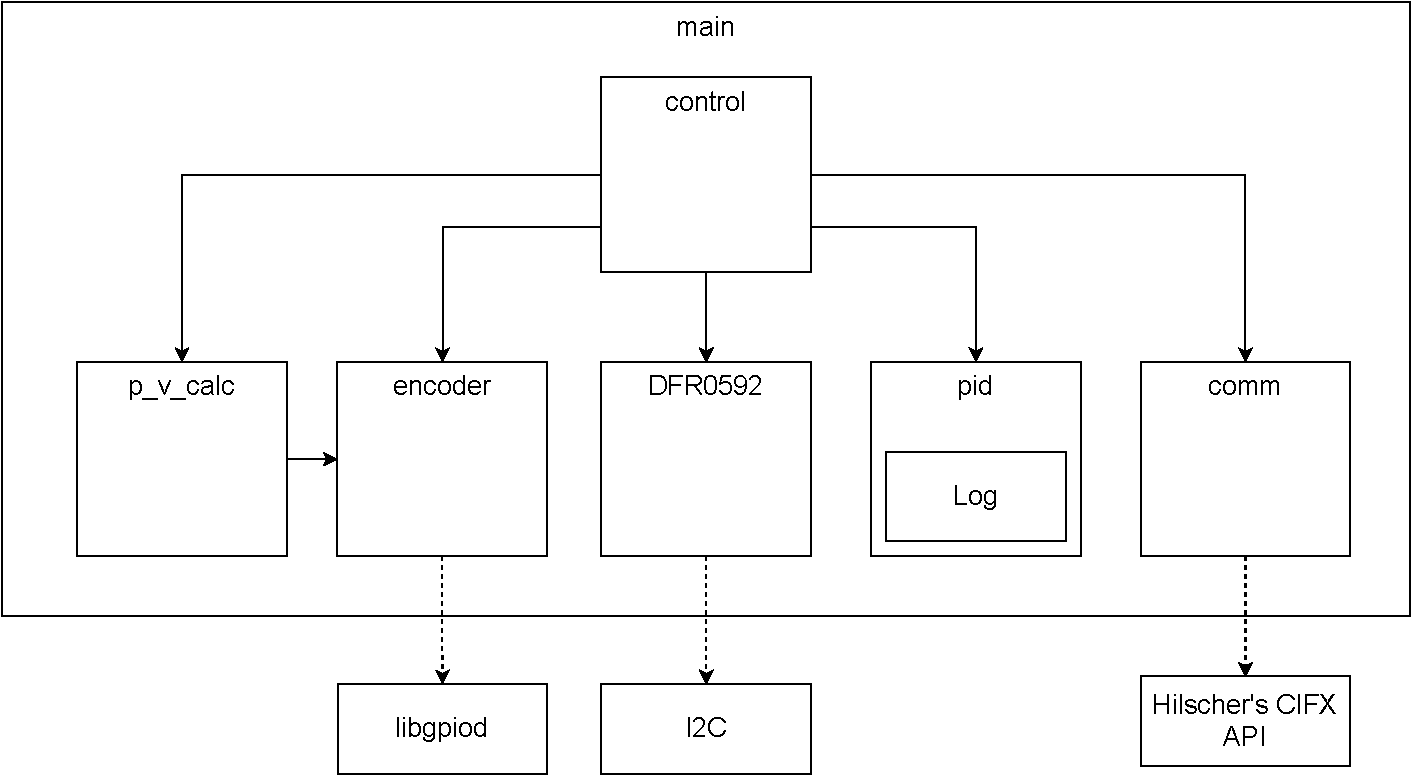
\includegraphics[width=0.8\linewidth]{sw-architecture.pdf}
	\caption{Overview of the slave device's software architecture}
	\label{fig:sw-architecture}
\end{figure}

The \verb|main| module will take care of initialising all data structures and sending the terminate commands when the user wishes to close the control application.
Configuration parameters can be passed as command-line arguments to the main module, which will be parsed and used during the run-time.
This module will serve as the entry point for the control application, where, after compilation, all modules will be integrated into a single executable.

The \verb|control| module will contain the function calls that determine the behaviour of the slave device during normal operation.
The run-time behaviour takes into consideration all parameters provided when launching the application.
It also takes care of moving data around between the other modules before calling functions that require some external data.
For example, the \verb|pid| module requires the set-point and plant feedback values, which are retrieved from the \verb|p_v_calc| module and \verb|comm| module, respectively.

The \verb|p_v_calc| module will be responsible for computing the motor velocity and position, based on an encoder counter.
Such counter is implemented on the \verb|encoder| module, which will convert the encoder signals onto a counter value.
In order to have access to the encoder signal, which will be connected to the GPIO header, we used the external library called \verb|libgpiod| to gain access to the GPIO pins.

The \verb|DFR0592| module is responsible for implementing functions to access and interface the DC motor control board.
All communication is done via I2C, which requires the usage of an external library.
In this particular implementation, we used the default Linux kernel I2C library.

The \verb|pid| module implements a discrete-time PID controller used for the local control of the motor's position or velocity.
Additionally, because all relevant data that describes the system performance is already contained in the PID data structure, we implemented the functionality of exporting such data on this module.

At last but not least, the \verb|comm| module will be responsible to make API calls to the RTE interface board driver, called \verb|CIFX|, in order to configure the RTE network and retrieve/send cyclic process data.
All the necessary steps to initialise, configure and manage the different RTE networks will already be implemented in the \verb|comm| module functions.
